\documentclass[12pt]{article}
\usepackage{fancyhdr}
\usepackage{amsmath}
\usepackage{amsthm}
\usepackage{mathtools}
\usepackage{enumitem}
\usepackage[Export]{adjustbox}
\usepackage{cancel}
\usepackage{algorithm}
\usepackage{bigints}
\usepackage[noend]{algpseudocode}
\usepackage{graphicx}
\usepackage[margin = 1in]{geometry}
\usepackage{blindtext}
\usepackage[section]{placeins}
\usepackage{xcolor,listings}
\usepackage{hyperref}
\usepackage{textcomp}
\usepackage{makecell}
\usepackage[utf8]{inputenc}
\usepackage[romanian]{babel}
\lstset{upquote=true}
\lstdefinestyle{myCustomRStyle}{
	language=R,
	backgroundcolor = \color{lightgray!10!white},
	numbers=left,
	stepnumber=1,
	numbersep=10pt,
	tabsize=2,
	showspaces=false,
	breaklines=true
	showstringspaces=false,
	basicstyle=\footnotesize\ttfamily,
	keywordstyle=\bfseries\color{blue!50!black},
	commentstyle=\itshape\color{orange!60!black},
	identifierstyle=\color{black},
	stringstyle=\color{green!50!black},
	xleftmargin=\parindent,
	frame=L
}
\lstset{literate=%
	*{0}{{{\color{blue}0}}}1
	{1}{{{\color{blue}1}}}1
	{2}{{{\color{blue}2}}}1
	{3}{{{\color{blue}3}}}1
	{4}{{{\color{blue}4}}}1
	{5}{{{\color{blue}5}}}1
	{6}{{{\color{blue}6}}}1
	{7}{{{\color{blue}7}}}1
	{8}{{{\color{blue}8}}}1
	{9}{{{\color{blue}9}}}1
}

\lstset{basicstyle=\small,style=myCustomRStyle}
\usepackage{amsfonts}
\graphicspath{ {./images/} }



\pagestyle{fancy}
\fancyhead{}
\fancyfoot{}
\usepackage[T1]{fontenc}
\fancyhead[L]{Pachetul contRV}
\fancyhead[R]{Proiect PS, grupa 244}
\setlength{\headheight}{25pt}
\fancyfoot[C]{\thepage}
\title{Pachet pentru lucru cu variabile aleatoare continue}
\author{Țânțaru Dragoș-Constantin, Vasiliu Florin \\Vintilă Eduard-Ionuț, Ristea Mihai-Cristian\\Grupa 244}

\begin{document}
\maketitle
\section{Introducere} \hfill \\
\indent Pachetul oferă un set de operații uzuale în lucrul cu variabile aleatoare continue, de la calcularea diverselor probabilități, la determinarea densităților condiționate și chiar la animații cu graficele unor repartiții cunoscute. Mai exact, pachetul permite:
\begin{itemize}
	\item construirea unui obiect de tip variabilă aleatoare continuă, unidimensională sau bidimensională, cu suport configurabil de utilizator
	\item calcularea probabilităților, printr-un apel de forma $P(X <= x)$ (avem implementate operațiile $<$, $<=$, $>$, $>=$, $==$)
	\item calcularea probabilităților condiționate de forma $P(X \ \mathrm{op_1} \ x_1 \ | \ X \ \mathrm{op_2} \ x_2)$, unde $\mathrm{op_1}$ și $\mathrm{op_2}$ sunt oricare din operațiile definite mai sus
	\item calcularea probabilităților condiționate de forma $P(X \ \mathrm{op} \ x \ | \ Y == y)$, unde Y e orice variabilă aleatoare continuă și op, din nou, orice operație de mai sus
	\item calcularea mediei, dispersiei și momentelor centrate sau inițiale ale unei variabile aleatoare continue
	\item aplicarea unor funcții continue asupra variabilelor aleatoare continue și prelucrarea rezultatelor obținute
	\item afișarea graficelor a diverselor repartiții și densități obișnuite
	\item observarea efectelor parametrilor asupra densității beta prin intermediul unei animații programate în R
	\item afișarea unor fișe de sinteză despre repartițiile și densitățiile obișnuite
	\item și multe alte funcționalități pe care le-am detaliat în documentație
\end{itemize} \hfill \\
\indent În mod specific, am rezolvat cerințele 1, 2, 3, 4, 5, 6, 7, 8, 10 și 11 din cerințele proiectului 1. \\
\indent Dificultățile cele mai importante întâmpinate la implementarea proiectului au fost folosirea eficientă a funcției $integrate$ și gestionarea corectă a variabilelor R, în contextului scoping-ului făcut de R (problemă explicată în detaliu la documentația pentru exercițiul 5). Pe scurt, pe prima am depășit-o scriind o funcție specifică pachetului $integrala$, care face suma integralelor pe suportul variabilelor și aplicând funcția $Vectorize$ asupra tuturor funcțiilor pe care le-am integrat, iar a doua folosind o funcție de tip „factory”. \\
\indent Principala limitare a pachetului este tipul de densități comune cu care poate lucra. Deoarece nu am reușit să găsim un mod bun de a stoca suporturi care nu sunt reuniuni de dreptunghiuri $[a, b] \times [c, d]$, pachetul nu permite lucrul cu variabile bidimensionale care au suporturi în care ori $x$, ori $y$ sunt definite pe intervale care depind de cealaltă variabilă. A nu se înțelege că nu se poate lucra cu variabile aleatoare continue dependente, problema apare doar când una dintre variabilele aleatoare are suportul dependent de cealaltă. În schimb, dacă suportul e de forma $\displaystyle \bigcup\limits_{i} ([a_i, b_i] \times [c_i, d_i])$, unde niciuna dintre $a_i, b_i, c_i, d_i$ nu depinde de $x$ sau $y$, se poate folosi fără probleme pachetul. \\
\indent În continuare, vom lua fiecare exercițiu pe rând și vom documenta implementarea, ideea de rezolvare și problemele întâmpinate. \\

\section{Cerința 1}	\hfill \\
\indent \textbf{1) Fiind dată o funcție f , introdusă de utilizator, determinarea unei constante de
	normalizare k. În cazul în care o asemenea constantă nu există, afișarea unui mesaj
	corespunzător către utilizator}\vspace{5mm}

\indent Scurtă descriere a antetului funcției: \\
\begin{center}
	\begin{tabular}{|| c | c | c ||}
		\hline
		Parametrul & Tipul & Descriere \\
		\hline
		\textcolor{blue}{Func} & \textcolor{violet}{function} & Funcția data ca parametru \\
		\hline
		\textcolor{blue}{sup} & \textcolor{violet}{listă de liste} & Suportul funcției \\
		\hline
	\end{tabular}
\end{center}\hfill \pagebreak
\begin{lstlisting}
	Nor_constant <- function(Func, sup) {
		
		sum <- 0
		
		for (i in sup) {
			tryCatch(
			sum <- sum + integrate(Vectorize(Func), i[1], i[2], abs.tol = 0)$value,
			error= function(err) {
				stop("Integrala e divergenta sau functia nu e integrabila") # daca integrala nu poate fi calculata returnez un mesaj de eroare
			}
			)
			
			if (i[1] == -Inf && i[2] == Inf) {
				i[1] <- -1000
				i[2] <-  1000
			}
			else if (i[1] == -Inf)
			i[1] <- i[2] - 1000
			else if (i[2] ==  Inf)
			i[2] <- i[1] + 1000
			
			if(any(sapply(seq(i[1], i[2], length.out = 1000), Func) < 0))
			stop("Functie negativa") # daca functia are valori negative nu pot calcula constanta de normalizare
			
		}
		
		if(sum == 0)
		stop("Nu exista constanta de normalizare pentru functia data") # daca integrala = 0 inseamna ca nu exista constanta de normalizare
		
		const <- 1 / sum
		return (const)
		
	}
\end{lstlisting}

\indent Va fi parcurs suportul funcției dată ca parametru, și vom calcula suma pe fiecare interval din suport. În același timp, verificăm dacă funcția e pozitivă pe fiecare interval din suport, folosind $any(sapply(seq(i[1], i[2], length.out = 1000), Func) < 0)$, pentru a alege 1000 de valori echidistante.\hfill \\
\indent La final, dacă integrala este 0 înseamnă că nu există constantă de normalizare și afișează un mesaj corespunzător. În caz contrar, calculează constanta și o returnează.\hfill \\


	\section{Cerința 2}
\textbf{2) Verificarea dacă o funcție introdusă de utilizator este densitate de probabilitate.}\vspace{5mm}

Dificultate întâmpinată: funcția \lstinline|integrate| returnează valori eronate pentru integranzi cu valoarea $0$ într-o mare parte a domeniului. Ca remediu, am ales să transmitem printr-un parametru suportul funcției de integrat (detalii în comentariul din cod).\par
De asemenea, în cazul funcțiilor pe ramuri, \lstinline|Vectorize()| devine o necesitate: evaluarea condițiilor din if-uri (de exemplu, $x > 0$) ia în considerare doar primul element al vectorului Boolean $x > 0$. Apare astfel conflict cu modul de lucru al procedurii \lstinline|integrate|, care evaluează funcția-argument pe un vector de mostre, nu punct-cu-punct.\par
Definiția funcției este următoarea: \\

\begin{lstlisting}
	# Suportul functiei f este reuniunea intervalelor specificate prin parametrul
	# sup - o lista de vectori de cate doua elemente, reprezentand extremitati de
	# interval. f este densitate de probabilitate - deci dp(f, sup)==TRUE - daca:
	# a) f(x) >= 0 pentru orice x din suport,
	# b) suma integralelor de f peste fiecare interval din sup este 1.
	
	# Din documentatia pentru integrate: "f must accept a vector of inputs and
	# produce a vector of function evaluations at those points". Considerand ca
	# utilizatorul introduce functia dorita in regim scalar -> scalar, aplicand
	# Vectorize() se obtine argumentul dorit pentru integrate.
	dp <- function(f, sup) {
		
		sum <- 0
		for (i in sup) {
			tryCatch(
			sum <- sum + integrate(Vectorize(f), i[1], i[2], abs.tol = 0)$value == 1,
			error = function(e) {
				print(sprintf("Integrala divergenta in intervalul [%.2f, %.2f]!", i[1], i[2]))
				return(FALSE)
			})
			
			if (i[1] == -Inf && i[2] == Inf) {
				i[1] <- -1000
				i[2] <-  1000
			}
			else if (i[1] == -Inf)
			i[1] <- i[2] - 1000
			else if (i[2] ==  Inf)
			i[2] <- i[1] + 1000
			
			if (any(sapply(seq(i[1], i[2], length.out = 1000), f) < 0)) {
				print(sprintf("Valoare negativa in intervalul [%.2f, %.2f]!", i[1], i[2]))
				return(FALSE)
			}
		}
		sum == 1
	}
\end{lstlisting}\vspace*{3\baselineskip} 

Exemple:
\begin{lstlisting}[numbers=none]
	> dp(function(x) 3*x^2, list(c(0, 1)))
	[1] TRUE
	
	> f <- function(x) if (x < 0) 1 + x else 1 - x
	> dp(f, list(c(-1, 1)))
	[1] TRUE
	
	> dp(function(x) x, list(c(1, 3), c(-1, 0)))
	[1] "Valoare negativa in intervalul [-1.00, 0.00]!"
	[1] FALSE
	
	> dp(function(x) x, list(c(0, Inf)))
	[1] "Integrala divergenta in intervalul [0.00, Inf]!"
	[1] FALSE
\end{lstlisting} \pagebreak

	\section{Cerința 3}
\textbf{3) Crearea unui obiect de tip variabilă aleatoare continuă pornind de la o densitate de
	probabilitate introdusă de utilizator. Funcția trebuie să aibă opțiunea pentru variabile
	aleatoare unidimensionale și respectiv bidimensionale.}\vspace{5mm}

Pentru a facilita lucrul cu variabile aleatoare continue atât unidimensionale, cât si bidimensionale, am definit clasa de tip S4 numită \textbf{contRV}. Toate instanțele acestei clase vor reține o mulțime de informații necesare pentru a efectua diverse operații pe variabile aleatoare continue. Mai precis, fiecare obiect \textbf{contRV} va avea 
asociat:
\begin{itemize}
	\item O densitate de probabilitate.
	\item Repartiția variabilei aleatoare continue
	\item Un Boolean ce indică dacă variabila aleatoare este bidimensională.
	\item Suportul densității de probabilitate. În cazul variabilelor unidimensionale, acesta este reprezentat de o listă de intervale închise. Pentru o v.a bidimensională $(X, Y)$, suportul este reținut sub forma unei liste ce conține suporturile lui $X$ și $Y$.
	\item Pentru o v.a unidimensională $X$, o referință către v.a bidimensională $(X, Y)$, în cazul in care $X$ s-a format în urma determinării densității marginale. Se folosește pentru a avea acces cu ușurință la densitatea comună în calculul unor probabilități ce implică pe $X$ și $Y$. 
\end{itemize}\vspace*{1\baselineskip} \par
Motivul pentru care este necesară specificarea suportului densității la crearea unui obiect de tip \textbf{contRV} este următorul: la calculul integralelor unde unul dintre capete nu este un număr finit, comportamentul funcției \lstinline|integrate()| poate produce rezultate neașteptate. Astfel, restricționând domeniul la punctele în care integrandul ia valori nenule, calculul integralei devine mult mai precis.
În stadiul actual însă, permitem ca suportul densitații să fie specificat doar ca o reuniune de intervale închise în cazul v.a unidimensionale, sau dreptunghiuri în cazul celor bidimensionale.\vspace*{1\baselineskip}\par

Definiția clasei este următoarea:
\begin{lstlisting}
	setClass("contRV", representation (
	densitate="function",
	val="function",
	bidimen="logical",
	suport="list",
	ref_va_bidimen = "contRV_or_NULL"
	))
	
	# Am folosit acest union pentru a permite referintei catre v.a bidimen sa fie nula
	setClassUnion("contRV_or_NULL", c("contRV", "NULL"))
\end{lstlisting}\pagebreak

Pentru a crea un obiect \textbf{contRV}, am definit următorul constructor:
\begin{lstlisting}
	contRV <- function(densitate, val = function(x) x, bidimen = FALSE, suport = list(c(-Inf, Inf)), ref_va_bidimen = NULL)
	{
		if(length(suport) < 2)
		suport <- list(suport, list())
		if (bidimen & missing(val))
		val = function(x, y) x * y
		
		obj <- new("contRV", densitate = densitate, val = val, bidimen = bidimen,
		suport = suport, ref_va_bidimen = ref_va_bidimen)
		
		return (obj)
	}
	
\end{lstlisting}

De exemplu, pentru crearea unui obiect \textbf{contRV} ce reprezintă o variabilă aleatoare continuă bidimensională $(X, Y)$ cu densitatea:
\[ 
f(x, y)= \left\{
\begin{array}{ll}
	\frac{6}{7}(x+y)^2, & (x, y) \in [0, 1] \times [0, 1] \\\\
	0,				   & \text{în rest}
\end{array} 
\right. 
\]
Scriem:
\begin{lstlisting}[numbers=none]
	XY <- contRV(densitate = function (x, y) 6/7(x+y)^2, bidimen = TRUE, suport = list(list(c(0, 1)), list(c(0, 1))))
\end{lstlisting}\vspace*{1\baselineskip}


De asemenea, clasa \textbf{contRV} pune la dispoziție utilizatorilor pachetului o colecție de metode pentru a efectua operații pe variabile aleatoare continue, precum: calculul probabilităților (cu ajutorul metodei $P$, detalii în exercițiul 7), calculul mediilor și a dispersiilor (metodele $E$ și $Var$, detalii în exercițiile 5-6) și obținerea densităților marginale (metodele $marginalaX$ și $marginalaY$). \pagebreak
	\section{Cerința 4}
\textbf{4) Reprezentarea grafică a densității și a funcției de repartiție pentru diferite valori ale
	parametrilor repartiției. În cazul în care funcția de repartiție nu este dată într-o formă
	explicită (ex. repartiția normală) se acceptă reprezentarea grafică a unei aproximări a acesteia}\vspace{5mm}

Oferim un set de funcții, câte două pentru fiecare repartiție (normală, exponențială, beta, gamma), care, pe baza parametrilor corespunzători, afișează densitatea sau funcția-repartiție. De exemplu, pentru a obține graficul densității în repartiția beta de parametri (2, 5), apelăm $den.beta(2, 5)$. Unele funcții conțin și valori implicite (repartiția normală este standard „by default” – la apel fără argumente).
Pentru repartiția beta, am adăugat și o funcție care afișează graficul densității animat: o buclă apelează succesiv \lstinline|plot|, urmat de un foarte scurt timp de așteptare, pentru cursivitatea animației. Graficul mișcător nu poate fi exportat însă; este funcțional în interiorul mediului RStudio. Detalii despre funcțiile densitate și repartiție în exercițiul 8. \\ \par
Funcțiile sunt definite astfel: \\

\begin{lstlisting}
	# Repartitia normala (implicit standard); m = medie, s = deviatie standard
	den.normala <- function(m = 0, s = 1) {
		curve(expr = 1 / (s * sqrt(2 * pi)) * exp(1) ^ (-(x - m)^2 / (2 * s^2)),
		from = m - 3 * s,
		to   = m + 3 * s,
		ylab = "densitate",
		main = "Densitatea in repartitia normala")
		abline(v = 0, col = "gray")
	}
	
	rep.normala <- function(m = 0, s = 1) {
		curve(expr = pnorm(x, m, s),
		from = m - 3 * s,
		to   = m + 3 * s,
		ylab = "probabilitate",
		main = "Functia repartitie normala")
	}
	
	# Repartitia exponentiala
	
	den.exponentiala <- function(l = 1) {
		curve(expr = l * exp(1) ^ (-l * x),
		from = 0,
		to   = 20,
		ylab = "densitate",
		main = "Densitatea in repartitia exponentiala")
	}
	
	rep.exponentiala <- function(l = 1) {
		curve(expr = 1 - exp(1) ^ (-l * x),
		from = 0,
		to   = 10,
		ylab = "probabilitate",
		main = "Functia repartitie exponentiala")
	}
	
	# Repartitia beta
	
	den.beta <- function(a, b) {
		curve(expr = x^(a - 1) * (1 - x) ^ (b - 1) /
		integrate(function(u) u^(a - 1) * (1 - u)^(b - 1),
		0, 1, abs.tol = 0)$value,
		from = 0,
		to   = 1,
		ylab = "densitate",
		main = "Densitatea in repartitia beta")
	}
	
	# Teste: den.beta(0.5, 0.5)
	#        den.beta(2, 2)
	#        den.beta(2, 5)
	
	# la fel, dar animata; a - fixat, 0 < b <= bmax
	den.beta_anim <- function(a = 2, bmax = 8) {
		
		par(bty = "o")
		
		for (b in seq(0.1, bmax, length.out = 150)) {
			
			d <- function(x) x^(a - 1) * (1 - x) ^ (b - 1) /
			integrate(function(u) u^(a - 1) * (1 - u)^(b - 1),
			0, 1, abs.tol = 0)$value
			
			x <- seq(0, 1, length.out = 1000)
			plot(x,
			d(x),
			type = "l",
			xlab = "x",
			ylab = "densitate",
			ylim = c(0, 7),
			main = "Densitatea in repartitia beta")
			
			legend(0.7, 6.5, legend = sprintf("b = %.2f", b), cex = 0.8)
			
			Sys.sleep(0.05)
		}
		
	}
	
	# Test: den.beta_anim()
	#       den.beta_anim(0.8, 15)
	
	rep.beta <- function(a, b) {
		curve(expr = pbeta(x, shape1 = a, shape2 = b),
		from = 0,
		to   = 1,
		ylab = "probabilitate",
		main = "Functia repartitie beta")
	}
	
	# Teste: rep.beta(5, 1)
	#        rep.beta(2, 2)
	#        rep.beta(2, 5)
	
	
	# Repartitia gamma; k - "shape", t - "scale"
	
	den.gamma <- function(k, t) {
		curve(expr = dgamma(x, shape = k, scale = t),
		from = 0,
		to   = 20,
		ylab = "densitate",
		main = "Densitatea in repartitia gamma")
	}
	
	# Teste: den.gamma(1, 2)
	#        den.gamma(2, 2)
	#        den.gamma(7.5, 1)
	
	rep.gamma <- function(k, t) {
		curve(expr = pgamma(x, shape = k, scale = t),
		from = 0,
		to   = 20,
		ylab = "probabilitate",
		main = "Functia repartitie gamma")
	}
	
	# Teste: rep.gamma(0.5, 1)
	#        rep.gamma(7.5, 1)
\end{lstlisting}
\begin{figure}[h!]
	\centering
	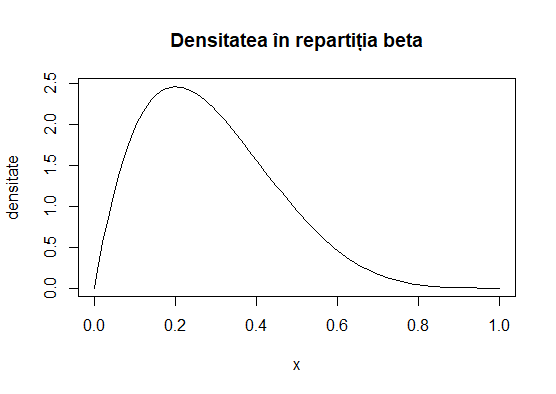
\includegraphics[scale=0.75]{DenBeta}
	\caption{den.beta(2, 5)}
\end{figure}

\begin{figure}[h!]
	\centering		
	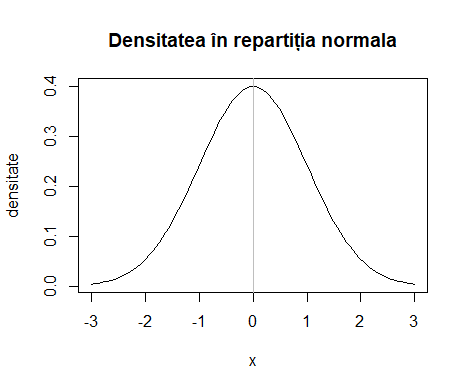
\includegraphics[scale=0.75]{DenNorm}
	\caption{den.normala(0, 1)}
\end{figure}

\begin{figure}
	\centering
	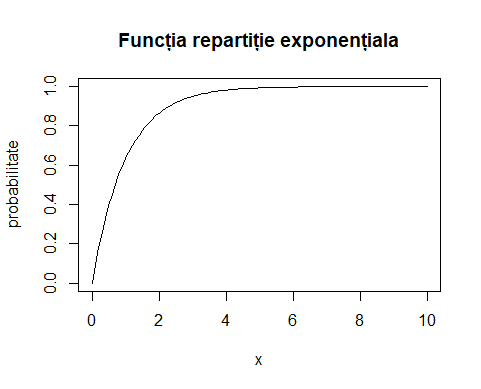
\includegraphics[scale=0.75]{RepExp}
	\caption{rep.exponentiala(1)}	
\end{figure}

\begin{figure}
	\centering
	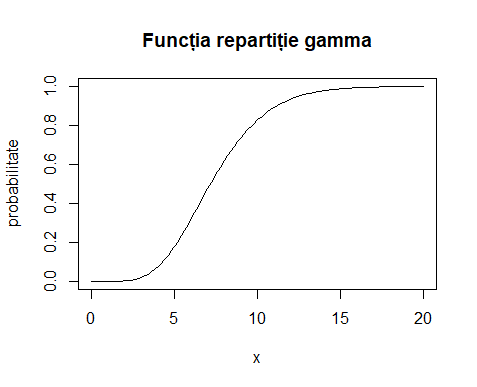
\includegraphics[scale=0.75]{RepGamma}
	\caption{rep.gamma(7.5, 1)}	
\end{figure} \pagebreak

\section{Cerința 5 + Cerința 6}
\textbf{\indent \indent5)Calculul mediei, dispersiei și a momentelor inițiale și centrate până la ordinul 4(dacă există). Atunci când unul dintre momente nu există, se va afișa un mesaj corespunzător către utilizator.\\
	\indent \indent6)Calculul  mediei și  dispersiei unei  variabile  aleatoare g(X), unde  X are  o repartiție continuă cunoscută iar g este o funcție continuă precizată de utilizator.} \\\\
\indent Toate funcțiile legate de aceste două cerințe au fost scrise având cazul general ca scop, ceea ce a a avut ca rezultat că am putut folosi aceleași funcții pentru calcularea mediei lui $X$, dar și lui $g(X)$ și chiar cuplurilor de forma $(X,Y)$, unde X și Y sunt două variabile aleatoare continue.\\

\subsection{Integrala}\hfill \\
\indent Înainte de a începe să prezentăm funcțiile relevante cerințelor, ar fi bine să explicăm ce face mai exact funcția $integrala$, folosită destul de mult de pachetul contRV. Mai întâi, o scurtă descriere a antetului funcției:
\begin{center}
	\begin{tabular}{|| c | c | c ||}
		\hline
		Parametrul & Tipul & Descriere \\
		\hline
		\textcolor{blue}{X} & \textcolor{violet}{contRV} & Variabila aleatoare pe care vrem să calculăm o integrală\\
		\hline
		\textcolor{blue}{dt} & \textcolor{violet}{integer} & \makecell{Variabila după care vrem să integrăm; \\este folosită explicit doar pentru determinarea densității\\ marginale, altfel implicit are valoarea 0 și se calculeaza\\ doar integrala densității variabilei aleatoare. Pentru dt = 1\\ se integrează doar după x, iar pentru dt = 2 doar după y.} \\
		\hline
	\end{tabular}
\end{center}\hfill \\
\indent Scopul parametrului $dt$ este doar să faciliteze calcularea densităților marginale, altfel poate fi ignorat.\\
\indent Funcția se uită mai întâi la ce fel de variabilă este X, unidimensională sau bidimensională. Să luăm mai întâi cazul unidimensionalei, care este cel mai ușor:
\begin{lstlisting}
	sum <- 0
	for (i in X@suport[[1]]) {
		tryCatch(sum <- sum + integrate(Vectorize(X@densitate), i[1], i[2], abs.tol = 1.0e-13)$value,
		error= function(err)
		{
			stop("Integrala a esuat.")
		})
	}
	return (sum)
\end{lstlisting}\hfill \\
\indent După cum se vede, este o simplă sumă pe intervalele din suport. O problemă pe care am întâmpinat-o în lucrul proiectului a fost fapul că pentru densități care sunt nenule pe intervale mici, funcția $integrate$ din R calculează eronat integralele. Astfel, avănd suportul salvat, putem evita complet această problemă. Valoarea din $abs.tol$ este $1.0e-13$ pentru că am observat că, din cauza erorilor de rotunjire ale float-urilor, $abs.tol = 0$ uneori returnează eroare, deși cu $abs.tol = 1.0e-13$ calculează corect integrala. Este posibil sa existe funcții care chiar și cu valoarea curentă să returneze eroare, dar noi n-am întâmpinat astfel de exemple.\\
\indent Acum să vedem cazul bidimensional, când vrem să calculăm integrala pe densitatea comună a unui cuplu de variabile aleatoare continue:
\begin{lstlisting}
	sum <- 0
	for(i in X@suport[[2]])
	{
		for(j in X@suport[[1]])
		{
			tryCatch(sum <- sum +
			integrate( function(y) {
				sapply(y, function(y) {
					integrate(function(x) X@densitate(x,y),j[1],j[2])$value
				})
			},i[1],i[2])$value,
			error= function(err)
			{
				stop("Eroare la integrarea densitatii.")
			})
		}
	}
	
	return(sum)
\end{lstlisting}\hfill \\
\indent După cum se vede, calculăm integrala pe $S_{X} \times S_{Y}$, unde am notat cu $S_{X}$ suportul lui $X$ din $(X, Y)$ si $S_{Y}$ suportul lui $Y$. Motivul pentru care am optat să calculăm pe întreg produsul cartezian este că, în cazul în care $X$ și $Y$ sunt independente, atunci suportul lui $(X, Y)$ va fi chiar $S_{X} \times S_{Y}$, fapt ce se vede din formula densității comune $f_{X,Y}(x,y) = f_{X}(x) \cdot f_{Y}(y)$. Dacă nu sunt independente, atunci oricum suportul lui $(X, Y)$ va fi sigur inclus în $S_{X} \times S_{Y}$, de exemplu, din formula densității marginale $\displaystyle f_{X}(x) = \int_{-\infty}^{\infty}f_{X,Y}(x,y)\mathrm{d}y$. Atunci, poate vom calcula niște integrale pe intervale în care densitatea comună este 0, dar câștigăm prin faptul că putem folosi același cod pentru două situații diferite, iar timpul pierdut de calcularea unor intervale nule este, în general, mic.\\
\indent Ultimul caz este cel în care vrem să extragem densitatea marginală. Vom prezenta doar cazul pentru densitatea marginală a lui Y, pentru că la X este identic. Codul:\\
\begin{lstlisting}
	#   Ok, deci ideea care mi a venit aici este sa construiesc un vector de functii asa:
	#   f_i+1 (y) = (integrala pe [a_i+1,b_i+1]dx) + f_i(y)
	
	funcs <- vector()
	factory <- function(i1, i2, pas)
	{
		i1; i2; pas; # pt closure
		if(pas == 1)
		{
			tmpF <-  Vectorize(function(y) {
				sapply(y, function(y) {
					integrate(function(x) X@densitate(x,y),i1,i2)$value
				})
			})
			funcs <<- c(funcs, tmpF)
		}
		else
		{
			tmpF <-  Vectorize(function(y) {
				sapply(y, function(y) {
					integrate(function(x) X@densitate(x,y),i1,i2)$value
				})
			})
			
			newF <- Vectorize(function(y){
				tmpF(y) + funcs[[pas - 1]](y)
			})
			funcs <<- c(funcs, newF)
		}
	}
	
	pas <- 0
	for(i in X@suport[[1]])
	{
		pas <- pas + 1
		factory(i[1], i[2], pas)
	}
	
	return(funcs[[length(funcs)]])
\end{lstlisting} \hfill \\
\indent Deoarece este posibil ca în formula $\displaystyle f_{Y}(y) = \int_{-\infty}^{\infty}f_{X,Y}(x,y)\mathrm{d}x$ suportul lui Y să fie spart în intervale, avem deja o problemă la construirea acestei funcții, pentru că va trebui să construim o funcție progresiv, calculând fiecare interval din suport. Soluția pe care am găsit-o este să folosim un vector de funcții, construit dupa următoarele reguli:
\begin{itemize}
	\item $\displaystyle f_1(y) = \int_{a_1}^{b_1}f_{X,Y}(x,y)\mathrm{d}x$, unde $a_1$ și $b_1$ sunt capetele primului interval din suportul lui Y
	\item $\displaystyle f_{i+1}(y) = \int_{a_{i+1}}^{b_{i+1}} f_{X,Y}(x,y)\mathrm{d}x + f_i(y)$, unde $a_{i+1}$ și $b_{i+1}$ sunt capetele primului celui de-al $i+1$-lea interval din suportul lui Y, iar $f_i(y)$ este functia rezultată din calcularea primelor $i$ integrale
\end{itemize}\pagebreak \par 
În final, în $f_n(y)$ o să avem densitatea marginală a lui Y, unde $n$ este numărul de intervale din suport.\\
\indent Încă o dificultate întâlnită a fost la creearea funcțiilor propriu-zise în R. Dacă nu am fi folosit funcția $factory$ și am fi pus direct codul ei în $for$, am observat că R nu salva corect valoarea lui $pas$ sau intervalele din $i$, ci în schimb punea peste tot ultimul $pas$, respectiv ultimul interval. Din ce am înteles, problema apare din cauza felului în care R implementează scoping-ul variabilelor. În orice caz, soluția noastră este inspirată din urmatorul răspuns: \url{https://stackoverflow.com/questions/12481404/how-to-create-a-vector-of-functions}. \hfill \\
\indent Sper că am clarificat destul de bine cum funcționează această funcție, de altfel fundamentală pentru implementarea clasei \textbf{contRV}, deoarece am încercat să folosim cât mai des funcția aceasta, în loc de $integrate$ singură.\\

\subsection{Media} \hfill \\
\indent Implementarea mediei se bazează pe formula ei obișnuită. Pentru aflarea mediei unei variabile continue $X$, recomandăm folosirea metodei $E(X)$, în loc de apelarea manuală a funcției $media(X)$.\\
\indent Antetul funcției arată astfel:
\begin{center}
	\begin{tabular}{|| c | c | c ||}
		\hline
		Parametrul & Tipul & Descriere \\
		\hline
		\textcolor{blue}{X} & \textcolor{violet}{contRV} & Variabila aleatoare căreia vrem să-i determinăm media\\
		\hline
	\end{tabular}
\end{center}\hfill \\
\indent Parametrul poate fi ori unidimensional, ori bidimensional, media este calculată corect în ambele cazuri. Media este implementată astfel: 
\begin{lstlisting}
	media <- function(X)
	{
		subIntegrala <- function(...)
		{
			X@val(...) * X@densitate(...)
		}
		
		subIntegrala <- Vectorize(subIntegrala)
		tmp <- contRV(densitate = subIntegrala, val = Vectorize(function(...) {retval <- 1}), bidimen = X@bidimen, suport = X@suport)
		
		tryCatch(retval <- integrala(tmp),
		error=function(err){
			stop("Media nu exista")
		}
		)
		return(retval)
	}
\end{lstlisting} \pagebreak \par
Codul poate arăta ciudat la prima vedere, probabil din cauza variabilei $tmp$.\\
\indent În primul rând, după cum se vede, am decis să folosim $\dots$ ca parametru pentru implementarea functiei „de sub integrală” a mediei, pentru a putea acoperi și cazul unidimensionalei, și bidimensionalei cu o singură funcție. Motivul pentru care am făcut funcția aceasta este și pentru că am considerat că avem un cod mai elegant dacă nu încărcăm câmpul „densitate” din constructorul lui $tmp$ cu o funcție definită pe loc.\\
\indent În al doilea rând, deoarece deja avem funcția $integrala$ care știe să calculeze o integrală pe un anumit suport, ar fi bine să o apelăm cumva, decât să rescriem aceiași secvență de cod de mai multe ori. Desigur, dacă am apela $integrala(X)$, nu am obține rezultatul corect, pentru că vrem să integrăm funcția $subIntegrala$, nu densitatea lui $X$. Atunci, am găsit soluția să folosim un fel de pseudo-variabilă, căreia îi dăm ca densitate funcția pe care vrem să o integrăm pentru a putea apela $integrala$ pe această pseudo-variabilă. Acest artificiu este folosit de mai multe ori în proiect, deoarece am întâmpinat mai multe situații asemănătoare, în care am fi putut folosi o funcție destinată doar variabilelor continue, pentru a calcula diverse valori.\\

\subsection{Dispersia} \hfill \\
\indent Dispersia seamănă ca implementare foarte mult cu media, doar că desigur diferă calculele făcute. De asemenea, există o metodă definită pentru dispersie, anume $Var(X)$. Antetul funcției arată astfel:
\begin{center}
	\begin{tabular}{|| c | c | c ||}
		\hline
		Parametrul & Tipul & Descriere \\
		\hline
		\textcolor{blue}{X} & \textcolor{violet}{contRV} & Variabila aleatoare căreia vrem să-i determinăm dispersia\\
		\hline
	\end{tabular}
\end{center}\hfill \\
\begin{lstlisting}
	dispersia <- function(X)
	{
		# formula clasica cu integrala
		
		tryCatch(m <- media(X), warning=function(wr)
		{
			stop("Calcularea dispersiei a esuat, media nu exista")
		})
		
		xCoef <- function(...)
		{
			
			X@val(...) - m
		}
		
		coefRaised <- powF(xCoef, 2)
		coefRaised <- Vectorize(coefRaised)
		
		subIntegrala <- function(...)
		{
			coefRaised(...) * X@densitate(...)
		}
		subIntegrala <- Vectorize(subIntegrala)
		tmp <- contRV(densitate = subIntegrala, val = Vectorize(function(...) {retval <- 1}), bidimen = X@bidimen, suport = X@suport)
		
		tryCatch(retval <- integrala(tmp),
		error= function(err)
		{
			stop("Dispersia nu exista.")
		})
		return(retval)
	}
\end{lstlisting}\hfill \\
\indent Cum spuneam, este calculată în mare ca media, folosind o funcție $subIntegrala$ și un pseudo-contRV $tmp$. Diferența majoră este introducerea funcției $xCoef$, care reprezintă $(x - E[X])$ din formulă. Voi discuta repede și despre funcția $powF$, care este foarte simplă de altfel. \\
\subsubsection{powF} \hfill \\
\indent Scopul acestei funcții este de a lua funcția $f$ din parametru și de a returna o funcție egală cu $f$ ridicată la o anumită putere, dată de asemenea ca parametru. Antetul:
\begin{center}
	\begin{tabular}{|| c | c | c ||}
		\hline
		Parametrul & Tipul & Descriere \\
		\hline
		\textcolor{blue}{f} & \textcolor{violet}{funcție} & Funcția pe care vrem să o ridicăm la putere\\
		\hline
		\textcolor{blue}{y} & \textcolor{violet}{integer} & Puterea\\
		\hline
	\end{tabular}
\end{center}\hfill \\
\indent Implementarea arată astfel:
\begin{lstlisting}
	powF <- function(f, y)
	{
		ret <- function(...)
		{
			f(...) ^ y
		}
	}
\end{lstlisting} \hfill \\
\indent Trebuie ținut cont de modul în care R face scoping, astfel că nu putem scrie ceva de genul:
\begin{lstlisting}
	func <- powF(func, 3)
	
	# Body-ul lui func este acum
	func <- function(...)
	{
		f(...) ^ y # atentie!! f este tot func, deci avem o recursie infinita
	}	
\end{lstlisting} \hfill \\
\indent Se poate evita ușor problema aceasta folosind o funcție $funcRaised$ în care să stocăm $powF(func, 3)$. Asta este și soluția folosită de noi în proiect.\\
\noindent\makebox[\linewidth]{\rule{\paperwidth}{0.4pt}}
\\\\
\indent Revenind la dispersie, după ce ridicăm $xCoef$ la puterea a 2-a, codul devine aproape identic ca la medie.\\

\subsection{Momentul centrat de ordin r}\hfill \\
\indent Momentul centrat este implementat într-o măsură asemănătoare. Să vedem mai întâi antetul:
\begin{center}
	\begin{tabular}{|| c | c | c ||}
		\hline
		Parametrul & Tipul & Descriere \\
		\hline
		\textcolor{blue}{X} & \textcolor{violet}{contRV} & Variabila aleatoare pe care vrem să calculăm momentul centrat\\
		\hline
		\textcolor{blue}{ordin} & \textcolor{violet}{integer} & Ordinul\\
		\hline
	\end{tabular}
\end{center}\hfill \\
\indent Implementarea este aproape identică cu dispersia, doar că acum ridicăm $xCoef$ la $r$, în loc de $2$. O modificare pe care am făcut-o a fost că, dacă $r < 3$, putem calcula momentul centrat în funcție de funcțiile deja scris în pachet în modul următor:
\begin{lstlisting}
	moment_centrat <- function(X, ordin)
	{
		# cazurile triviale
		if(ordin == 0)
		return(1)
		else if(ordin == 1)
		tryCatch({ # trebuie totusi verificat daca E(X) exista, ca altfel nu va da nici macar 0
			media(X)
			return(0)
		}, error= function(err)
		{
			stop(paste("Calcularea momentului centrat de ordin ", ordin, " a esuat, nu exista media."))
		})
		else if(ordin == 2)
		tryCatch({  # X dispersia nu exista, vrem un mesaj specific pt momente
			return(dispersia(X))
		}, error= function(err)
		{
			stop(paste("Calcularea momentului centrat de ordin ", ordin, " a esuat, nu exista dispersie."))
		})
		
		tryCatch(m <- media(X), warning=function(wr)
		{
			stop(paste("Calcularea momentului centrat de ordin ", ordin, " a esuat"))
		})
		
		xCoef <- function(...)
		{
			
			X@val(...) - m
		}
		
		coefRaised <- powF(xCoef, ordin)
		coefRaised <- Vectorize(coefRaised)
		
		subIntegrala <- function(...)
		{
			coefRaised(...) * X@densitate(...)
		}
		subIntegrala <- Vectorize(subIntegrala)
		tmp <- contRV(densitate = subIntegrala, val = Vectorize(function(...) {retval <- 1}), bidimen = X@bidimen, suport = X@suport)
		
		tryCatch(retval <- integrala(tmp),
		error= function(err)
		{
			stop(paste("Momentul centrat de ordin ", ordin, " nu exista."))
		})
		return(retval)
	}
\end{lstlisting} \hfill \\
\indent În cazurile "triviale", adică cele în care ne putem folosi de funcții deja scrise, am optat să le apelăm pentru a obține un comportament al funcțiilor cât mai apropiat de cel așteptat. De asemenea, momentele centrate și inițiale se apelează direct cu funcțiile lor, deoarece nu am avut vreo idee de cum să le definim un generic mai convenabil. \\
\subsection{Momente inițiale de ordin r}\hfill \\
\indent Codul este aproape identic cu cel al momentului centrat, doar ca $xCoef$ va fi doar $X@val(...)$. Antetul: 
\begin{center}
	\begin{tabular}{|| c | c | c ||}
		\hline
		Parametrul & Tipul & Descriere \\
		\hline
		\textcolor{blue}{X} & \textcolor{violet}{contRV} & Variabila aleatoare pe care vrem să calculăm momentul inițial\\
		\hline
		\textcolor{blue}{ordin} & \textcolor{violet}{integer} & Ordinul\\
		\hline
	\end{tabular}
\end{center}\hfill \\
\begin{lstlisting}
	moment_initial <- function(X, ordin)
	{
		# cazurile triviale
		if(ordin == 0)
		return(1)
		else if(ordin == 1)
		tryCatch({ # trebuie totusi verificat daca E(X) exista, ca altfel nu va da nici macar 0
			return(media(X))
		}, error= function(err)
		{
			stop(paste("Calcularea momentului initial de ordin ", ordin, " a esuat."))
		})
		
		
		xCoef <- function(...)
		{
			
			X@val(...)
		}
		
		coefRaised <- powF(xCoef, ordin)
		coefRaised <- Vectorize(coefRaised)
		
		subIntegrala <- function(...)
		{
			coefRaised(...) * X@densitate(...)
		}
		subIntegrala <- Vectorize(subIntegrala)
		tmp <- contRV(densitate = subIntegrala, val = Vectorize(function(...) {retval <- 1}), bidimen = X@bidimen, suport = X@suport)
		
		tryCatch(retval <- integrala(tmp),
		error= function(err)
		{
			stop(paste("Momentul initial de ordin ", ordin, " nu exista."))
		})
		return(retval)
	}
\end{lstlisting}

\subsection{Implementarea pentru exercițiul 6}\hfill \\
\indent Pentru a asigura faptul că funcțiile pot fi folosite și în situații de genul $g(X)$, am stocat repartiția lui X în câmpul $val$. De asemenea, am definit genericul $aplica$ care, după cum îi spune și numele, ia o funcție $g$ și o variabilă X și returnează o variabilă X', căreia i-am aplicat asupra repartiției $g$. Antetul lui $aplica$ este:
\begin{center}
	\begin{tabular}{|| c | c | c ||}
		\hline
		Parametrul & Tipul & Descriere \\
		\hline
		\textcolor{blue}{X} & \textcolor{violet}{contRV} & Variabila aleatoare\\
		\hline
		\textcolor{blue}{g} & \textcolor{violet}{funcție} & Funcția continuă pe care vrem să o aplicăm\\
		\hline
	\end{tabular}
\end{center}\hfill \\
\indent Deci, dacă vrem să aflăm, de exemplu, $E[g(X)]$, putem scrie $E(aplica(X, g))$ și, deoarece toate funcțiile de mai sus apeleaza câmpul $val$, sigur va funcționa. Dacă $g$ returnează efectiv un obiect contRV, putem apela direct $E(g(X))$. \\
\indent Codul lui $aplica$ este:\\\\
\begin{lstlisting}
	setMethod("aplica", "contRV",
	function(object, f){
		retval <- contRV(object@densitate, Vectorize(compunere(f, object@val)), object@bidimen, object@suport,
		ref_va_bidimen = object@ref_va_bidimen)
	})
\end{lstlisting}\hfill \\
\indent Iar compunere este definit:
\begin{lstlisting}
	compunere <- function(f, g)
	{
		function(...) f(g(...))
	}
\end{lstlisting} \pagebreak

	\section{Cerința 7}
\textbf{7) Crearea unei funcții P care permite calculul diferitelor tipuri de probabilități asociate
	unei variabile aleatoare continue(similar funcției P din pachetul discreteRV) }\vspace{5mm}

Pentru a calcula probabilități pe variabile aleatoare continue, am definit funcția $P$ ca o metodă a clasei \textbf{contRV}, astfel:
\begin{lstlisting}[numbers=none]
	setMethod("P", "contRV",
	function (object) {
		return (integrala(object)) # integreaza pe suport
	})
\end{lstlisting}

După cum se poate observa, parametrul funcției este un obiect de tip \textbf{contRV}. Acest lucru poate părea ciudat la prima vedere; ar fi inutil să putem calcula doar probabilități de tipul $P(X)$, intrucât rezultatul ar fi întodeauna egal cu 1. În contextul pachetului, însă, un obiect de tip \textbf{contRV} nu reprezintă întotdeauna o variabilă aleatoare propriu-zisă. Mai precis, orice obiect poate fi rezultatul unei expresii de tipul: $X \leq x$, $(X \leq x) \cap  (Y \geq y)$, $(X < a) \cup (X > b)$ etc. Astfel, prin evaluarea expresiilor, restrângem domeniul pe care integrăm densitățile în calculul probabilităților și să păstrăm notații cât mai apropiate de cele matematice(detalii în exemplele de la sfârșit).\par

Pentru a evalua expresiile, am supraîncărcat următorii operatori:
\begin{lstlisting}
	setMethod("<", c("contRV", "numeric"), function (e1, e2) {
		comp(e1, e2, "<=") # P(X < x) = P(X <= x)
	})
	setMethod("<=", c("contRV", "numeric"), function (e1, e2) {
		comp(e1, e2, "<=")
	})
	setMethod(">", c("contRV", "numeric"), function (e1, e2) {
		comp(e1, e2, ">=") # P(X > x) = P(X >= x)
	})
	setMethod(">=", c("contRV", "numeric"), function (e1, e2) {
		comp(e1, e2, ">=")
	})
	setMethod("==", c("contRV", "numeric"), function (e1, e2) {
		comp(e1, e2, "==")
	})
	setMethod("%AND%", c("contRV", "contRV"), function (e1, e2) {
	op(e1, e2, "&") # intersectie
})
setMethod("%OR%", c("contRV", "contRV"), function (e1, e2) {
op(e1, e2, "|") # reuniune
})
setMethod("|", c("contRV", "contRV"), function (e1, e2) {
cond(e1, e2) # conditionare
})
\end{lstlisting}\pagebreak

Pentru operatorii de inegalitate și egalitate, se observă ca aceștia au drept parametri un obiect \textbf{contRV} și un număr real. Se apelează funcția $comp$, ce va efectua restrângerea efectivă a suportului variabilei aleatoare pentru calculul probabilităților.

\begin{lstlisting}
# Determina suportul pentru expresii de tipul X <= x, X >= x
comp <- function(X, x, c)
{

if (X@bidimen)
stop("Nu se poate compara o v.a bidimensionala cu un numar real!")

suportNou <- list()
nr <- 1

# Presupunem ca intervalele sunt in ordine crescatoare dupa capatul inferior
# si nu se intersecteaza!	
if (c == "==")
{
	for (i in X@suport[[1]])
	{
		a <- i[1]
		b <- i[2]
		
		if (x < a)
		break # nu mai are rost sa cautam
		
		if (a <= x & b >= x) # daca x se afla in intervalul [a, b]
		{
			suportNou[[nr]] <- c(x, x) # suportul va fi intervalul [x, x]
			break
		}
	}
}
else if (c == "<=")
{
	# Exemplu: Daca suportul densitatii este format din [0, 2] U [4, 7] U [9, 11]
	# Noul suport pentru X <= 5 va fi [0, 2] U [4, 5]
	
	for (i in X@suport[[1]])
	{
		a <- i[1]
		b <- i[2]
		
		if (x < a)  # daca x este mai mic decat capatul inferior al intervalului
		break # am terminat de construit suportul
		
		if (a <= x & b >= x) # daca x se afla in intervalul [a, b]
		{
			suportNou[[nr]] <- c(a, x) # adaugam ultimul interval din noul suport, adica [a, x]
			break
		}
		
		# altfel, n-am ajuns la un interval care sa-l contina pe x, deci il adaugam in suportul nou
		suportNou[[nr]] <- c(a, b)
		nr <- nr + 1
	}
}
else # ">="
{
	# Exemplu: Daca suportul densitatii este format din [0, 2] U [4, 7] U [9, 11]
	# Noul suport pentru X >= 5 va fi [5, 7] U [9, 11]
	
	# parcurgem intervalele in ordine descrescatoare dupa capatul inferior
	for (i in rev(X@suport[[1]]))
	{
		a <- i[1]
		b <- i[2]
		
		if (x > b)
		break
		
		if (a <= x & b >= x) # daca x se afla in intervalul [a, b]
		{
			suportNou[[nr]] <- c(x, b) # adaugam ultimul interval din noul suport, adica [x, b]
			break
		}
		
		# altfel, inca n-am ajuns la un interval care sa-l contina pe x, deci il adaugam in suportul nou
		suportNou[[nr]] <- c(a, b)
		nr <- nr + 1
	}
	
	# inversam ordinea din noul suport, intrucat am parcurs intervalele din suport in ordine inversa
	suportNou <- rev(suportNou)
}

# atentie! rezultatul obtinut nu mai este o v.a! se foloseste doar pt a calcula probabilitati!
return (contRV(densitate = X@densitate, val = X@val, bidimen = X@bidimen, suport = suportNou,
ref_va_bidimen = X@ref_va_bidimen))
}
\end{lstlisting}\pagebreak

Pentru operatorii \%AND\% și \%OR\% ce implementează intersecția, respectiv reuniunea de variabile aleatoare continue, se apelează funcția $op$, care va avea un comportament diferit în funcție de relația dintre cei doi parametri $X$ și $Y$ de tip \textbf{contRV}. Mai exact, distingem următoarele cazuri:
\begin{itemize}
\item $X$ și $Y$ au aceeași densitate de probabilitate(apare de obicei în urma unor expresii de genul: $(X < a) \cap (X > b)$ ), caz în care formăm un obiect de tip \textbf{contRV} cu densitatea cunoscută și drept suport intersecția dintre suporturile lui $X$ și $Y$.
\item $X$ și $Y$ au o referință către aceeași v.a bidimensională, așa că formăm un nou obiect nou obiect \textbf{contRV} cu densitatea comună deja cunoscută și drept suport produsul cartezian intre suportul lui $X$ și cel al lui $Y$
\item $X$ și $Y$ au câte o referință către v.a bidimensionale diferite(sau nu au nicio referință), caz în care le considerăm independente și formăm un nou obiect \textbf{contRV} cu densitatea comună $f(x, y) = f_X(x) \cdot f_Y(y)$ și drept suport produsul cartezian intre suportul lui $X$ și cel al lui $Y$		
\end{itemize}

Funcția $op$ este definită astfel:
\begin{lstlisting}
# Reuniune si intersectie de variabile aleatoare
op <- function(X, Y, o)
{	
suportNou <- list()
nr <- 1

if (o == "&") # intersectie
{
	
	if (!identical(X@densitate, Y@densitate))
	{
		
		XY <- NULL
		
		if (!is.null(X@ref_va_bidimen) & identical(X@ref_va_bidimen, Y@ref_va_bidimen))
		{
			# aici se face o copie
			XY <- X@ref_va_bidimen
		}
		else
		{
			# consideram ca sunt independente
			XY <- contRV(densitate = function(x, y) {X@densitate(x) * Y@densitate(y)}, bidimen = TRUE)
		}
		
		XY@suport[[1]] <- X@suport[[1]]
		XY@suport[[2]] <- Y@suport[[1]]
		
		return (XY)
	}
	
	for (i in X@suport[[1]])
	{
		for (j in Y@suport[[1]])
		{
			# reuniuni de intersectii ale intervalelor din suport
			
			A <- interval_intersect(i, j)
			if (!is.null(A))
			{
				suportNou[[nr]] <- A
				nr <- nr + 1
			}
		}
	}
	
	return (contRV(densitate = X@densitate, val = X@val, bidimen = X@bidimen, suport = suportNou,
	ref_va_bidimen = X@ref_va_bidimen)) # intoarce contRV pt a integra suportul ramas
}
else # reuniune
{
	return (P(X) + P(Y) - P(X %AND% Y)) # aici intoarce deja probabilitatea calculata
	# problema este ca nu se mai pot aplica alte operatii pe v.a
}
}
\end{lstlisting}\par
O limitare a acestei funcții ar fi că în urma unei operații de reuniune, nu se întoarce un obiect \textbf{contRV} pentru a fi folosit în alte expresii, ci direct rezultatul probabilitații, adică $P(X \in A) + P(Y \in B) - P(X \in A, Y \in B)$.\vspace*{2\baselineskip}\par

Ultimul operator implementat este cel de condiționare:
\begin{lstlisting}[numbers=none]
setMethod("|", c("contRV", "contRV"), function (e1, e2) {
cond(e1, e2)
})
\end{lstlisting}

pentru care se apelează funcția $cond$, care are la rândul ei un comportament diferit în funcție de relația dintre cele 2 obiecte $X$ și $Y$ de tipul \textbf{contRV}. Dacă:
\begin{itemize}
\item $X$ și $Y$ au densitățile marginale dintr-o v.a bidimensională $(X, Y)$, atunci calculează direct probabilitatea folosind formula: $\displaystyle P(X \in A \mid Y = y) = \int_{A} f_{X|Y}(x|y) \,dx$, unde densitatea condiționată o obținem din funcția \texttt{dens\_condit\_x\_de\_y}, descrisă în exercițiul 11.
\item Altfel, avem ori $X$ și $Y$ independente, ori au aceeași densitate. În ambele cazuri, putem folosi formula: $\displaystyle P(X \in A \mid Y \in B) = \frac{P(X \in A, Y \in B)}{P(Y \in B)}$. Chiar și pentru $X$, $Y$ independente, rezultatul ar fi cel așteptat, adică $P(X \in A)$.
\end{itemize}\pagebreak

Funcția \texttt{cond} arată în felul următor:
\begin{lstlisting}
# Calculeaza probabilitatea conditionata
# X si Y pot fi expresii de tipul Z <= x, Z %AND% W etc.
cond <- function (X, Y)
{
if (!is.null(X@ref_va_bidimen) & identical(X@ref_va_bidimen, Y@ref_va_bidimen))
{
	# aici probabil ar trebui verificat daca X si Y referintiaza aceeasi v.a bidimensionala
	XY <- X@ref_va_bidimen
	fx_cond_y <- dens_condit_x_de_y(XY)
	
	if (length(Y@suport[[1]]) == 0) # inseamna ca nu a fost gasit y in suportul lui Y
	{
		return (0)
	}
	
	if (length(Y@suport[[1]]) != 1  || Y@suport[[1]][[1]][[1]] != Y@suport[[1]][[1]][[2]])
	{
		stop("Nu pot calcula asa ceva! Suportul lui Y trebuie sa fie un singur punct!!")
	}
	
	
	yfixat <- Y@suport[[1]][[1]][[1]]
	
	sum <- 0
	for (i in X@suport[[1]]) {
		tryCatch(sum <- sum + integrate(fx_cond_y, i[1], i[2], y = yfixat, abs.tol = 1.0e-13)$value,
		error= function(err)
		{
			stop("Integrala a esuat.")
		})
	}
	return (sum)
	
}
else
{
	return (integrala(X %AND% Y) / integrala(Y)) # P(X intersect Y) / P(Y)
}
}
\end{lstlisting}\pagebreak

Comparație între notații:
\begin{center}
\begin{tabular}{|| c | c ||}
\hline
\textcolor{blue}{contRV} & \textcolor{violet}{Notație matematică} \\

\hline
\lstinline|P(X <= x)| & $P(X \leq x)$ \\

\hline
\lstinline|P((X <= a)  %AND% (Y >= b))| & $P(X \leq a, Y \geq b)$ \\

\hline
\lstinline|P((X <= a)  %OR% (X >= b))| & $P(X \leq a \cup X \geq b)$ \\


\hline
\lstinline!P((X >= a)  %AND% (X <= b)  | X < c) ! & $P(a \leq X \leq b \mid X < c)$ \\

\hline
\lstinline!P(X > x | Y == y)! & $P(X > x \mid Y = y)$ \\

\hline

\end{tabular}
\end{center}\vspace*{3\baselineskip}

Exemple de cod:
\begin{lstlisting}[numbers=none]
> XY <- contRV(densitate = function (x, y) (6/7) * (x+y)^2,
bidimen = TRUE,
suport = list(list(c(0, 1)), list(c(0, 1))))
> X <- marginalaX(XY)
> Y <- marginalaY(XY)
> P((X <= 0.5) %AND% (X >= 0.2) | Y == 0.2)
[1] 0.1622093
> P((X <= 0.7) %AND% (Y >= 0.5))
[1] 0.3815


> func <- function(x)
+ {
if (x < -1)
0
else if (x < 0)
1 + x
else if (x < 1)
1 - x
else
0
}
> Z <- contRV(densitate = Vectorize(func), bidimen = FALSE, suport = list(c(-1, 1)))
> P(Z <= 0)
[1] 0.5
> P(((Z <= 0.5) %AND% (Z >= -0.7)) %OR% (Z <= 1))
[1] 1
\end{lstlisting} \pagebreak

	\section{Cerința 8}
\textbf{8.) Afișarea unei “fișe de sinteză” care să conțină informații de bază despre respectiva
	repartiție(cu precizarea sursei informației!). Relevant aici ar fi să precizați pentru ce e
	folosită in mod uzual acea repartiție, semnificația parametrilor, media, dispersia etc.}\vspace{5mm}\\
\indent Scurtă descriere al antetului funcției: \\
\begin{center}
	\begin{tabular}{|| c | c | c ||}
		\hline
		Parametrul & Tipul & Descriere \\
		\hline
		\textcolor{blue}{Rep}	 & \textcolor{violet}{Unul din vectorii definiți în pachet} & Repartiția dată ca parametru \\
		\hline
	\end{tabular}
\end{center}	
\begin{lstlisting}
	#Functia afiseaza informatiile despre o repartitie mai compact
	#compact = fara spatii goale
	#De asemenea reprezinta o metoda mai intuitiva de a afisa
	Fisa_sinteza <- function(Rep){
		for (i in Rep)
		{
			print(i)
		}
		
	}
\end{lstlisting}


Funcția Fisa\underline{\hspace{.08in}}sinteza afișează informațiile salvate despre repartiția dată ca parametru sub forma unei fișe de sinteză.\hfill \break
\indent Informațiile sunt salvate într-o listă de elemente de tip String. Avem următoarele liste ce pot fi afișate:
\begin{itemize}
	\item rep\_uniforma
	\item rep\_exponentiala
	\item rep\_normala
	\item rep\_gamma
	\item rep\_beta
	\item rep\_X2 (X stă în loc de $\chi$, pentru a nu avea erori de encoding)
	\item rep\_student
\end{itemize} \pagebreak

	\section{Cerința 10}
\textbf{10) Calculul covarianței și coeficientului de corelație pentru două variabile aleatoare
	continue(Atenție: Trebuie să folosiți densitatea comună a celor două variabile
	aleatoare!)
}\vspace{5mm}

\subsection{Covarianță}
\begin{center}
	\begin{tabular}{|| c | c | c ||}
		\hline
		Parametrul & Tipul & Descriere \\
		\hline
		\textcolor{blue}{Z} & \textcolor{violet}{contRV} & Variabila aleatoare continuă bidimensională $Z = (X, Y)$ \\
		
		\hline
	\end{tabular}
\end{center}\hfill \\

Funcția \texttt{Cov} calculează covarianța pe baza formulei:
\begin{equation*}
	Cov(X, Y) = E[XY] - E[X] \cdot E[Y]
\end{equation*}

\begin{lstlisting}
	Cov <- function(Z) {
		
		if (!Z@bidimen) {
			print("Variabila nu este bidimensionala!")
			NA
		}
		else {
			
			X <- marginalaX(Z)
			Y <- marginalaY(Z)
			
			return (E(Z) - E(X) * E(Y))
			
		}
	}
\end{lstlisting}

\subsection{Coeficientul de corelație}
\begin{center}
	\begin{tabular}{|| c | c | c ||}
		\hline
		Parametrul & Tipul & Descriere \\
		\hline
		\textcolor{blue}{Z} & \textcolor{violet}{contRV} & Variabila aleatoare continuă bidimensională $Z = (X, Y)$ \\
		
		\hline
	\end{tabular}
\end{center}\hfill \\

Funcția \texttt{Cor} calculează coeficientul de corelație pe baza formulei:
\begin{equation*}
	\rho(X, Y) = \frac{Cov(X, Y)}{\sqrt{Var(X) \cdot Var(Y))}}
\end{equation*}\pagebreak

\begin{lstlisting}
	Cor <- function(Z)
	{
		if (!Z@bidimen) {
			print("Variabila nu este bidimensionala!")
			NA
		}
		else {
			
			X <- marginalaX(Z)
			Y <- marginalaY(Z)
			
			return (Cov(Z) / sqrt(Var(X) * Var(Y)))
			
		}
	}
\end{lstlisting}\vspace*{2\baselineskip}

Exemple:
\begin{lstlisting}
	> Z <- contRV(densitate = function (x, y) (6/7) * (x+y)^2,
	bidimen = TRUE,
	suport = list(list(c(0, 1)), list(c(0, 1))))
	> Cov(Z)
	[1] -0.008503401
	> Cor(Z)
	[1] -0.1256281
\end{lstlisting} \pagebreak
\section{Cerința 11}
\textbf{11) Pornind  de  la  densitatea  comună  a  două  variabile  aleatoare  continue,  construirea densităților marginale și a densităților condiționate.} \hfill \\
\indent Implementarea densitățiilor marginale și condiționate se fac în funcție de funcția $integrala$. Astfel, avem densitățiile marginale:
\begin{lstlisting}
	# construieste o v.a continua pornind de la densitatea marginala a lui X in v.a bidimen (X, Y)
	marginalaX <- function(XY)
	{
		return (contRV(densitate = integrala(XY, 2), suport = XY@suport[[1]], bidimen = FALSE, ref_va_bidimen = XY))
	}
	
	# construieste o v.a continua pornind de la densitatea marginala a lui Y in v.a bidimen (X, Y)
	marginalaY <- function(XY)
	{
		return (contRV(densitate = integrala(XY, 1), suport = XY@suport[[2]], bidimen = FALSE, ref_va_bidimen = XY))
	}
\end{lstlisting} \hfill \\
\indent Câmpul $ref\_va\_bidimen$ este folosit pentru a putea accesa cuplul $(X, Y)$ din $X$ sau $Y$ când vrem să calculăm vreo probabilitate care le include pe ambele. \\
\indent Densitățiile condiționate au fost implementate în mod asemănător:
\begin{lstlisting}
	dens_condit_x_de_y <- function(Z)
	{
		dens_marginala_y <- integrala(Z,1)
		f <- function(x,y) {if (dens_marginala_y(y) != 0) {Z@densitate(x,y) / dens_marginala_y(y)} else stop("Densitatea marginala este 0")}
		return (Vectorize(f))
	}
	
	dens_condit_y_de_x <- function(Z)
	{
		dens_marginala_x <- integrala(Z,2)
		f <- function(x,y) {if (dens_marginala_y(y) != 0) {Z@densitate(x,y) / dens_marginala_x(x)} else stop("Densitatea marginala este 0")}
		return (Vectorize(f))
	}
\end{lstlisting} \pagebreak


\section{Concluzii} \hfill
\par Pachetul \textbf{contRV} oferă posibilitatea de a efectua diverse calcule probabilistice cu variabile aleatoare continue, folosind o sintaxă apropiată de cea matematică. Acoperă un set mare de cazuri care pot apărea în lucru cu probabilități, iar rezultatele sunt precise, având o eroare maximă de $1.0e-13$.
\subsection{Surse de inspirație}
\begin{itemize}
	\item \url{https://stackoverflow.com/questions/12481404/how-to-create-a-vector-of-functions}
	\item \url{https://online.stat.psu.edu/stat414/lesson/20/20.1}
	\item \url{https://en.wikipedia.org/wiki/Joint_probability_distribution}
	\item \url{https://stat.ethz.ch/pipermail/r-help/2013-February/347686.html}
	\item \url{http://cs.unitbv.ro/~pascu/stat/Distributii%20continue%20clasice.pdf%7D}
	\item \url{http://math.etc.tuiasi.ro/rstrugariu/cursuri/SPD2015/c7.pdf%7D}
	\item \url{http://images.wikia.com/nccmn/ro/images/3/37/Capitolul_10_REPARTITII_CLASICE.pdf%7D}
	\item \url{https://www.probabilitycourse.com/chapter5/5_2_3_conditioning_independence.php}
	\item \url{https://ro.qaz.wiki/wiki/Normalizing_constant}
	\item \url{https://rdrr.io/cran/discreteRV/f/}
	\item \url{https://rdrr.io/rforge/distr/}
\end{itemize}
\end{document}
